\chapter{Proposed Algorithms}\label{proposedalgo}
\section{Overview}\label{proposedoverview}
From the previous chapter, we have introduced a very fast point-to-point algorithm \textit{Polyanya}, 
in this chapter, we discuss how to effectively adapt \textit{Polyanya} for OkNN settings where
there are multiple candidate targets. In section~\ref{prob}, we introduce formal problem
statement and math notations; in section~\ref{mot}, we introduce two less efficient but very
straightforward solution to show the motivations of our proposed research;
section~\ref{intervalh} and \ref{targeth} present our research works which discuss the design of our algorithms and the correctness in theory.

\section{Problem Statement}\label{prob}
OkNN is a spatial query in two dimensions that can be formalised as follows:
\begin{definition}{Obstacle k-Nearest Neighbour (OkNN):}\newline
Given a set of points $T$, a set of obstacles $O$, a distinguished point $q$ and and an integer $k$: 
\textbf{return} a set $\text{kNN} = \{t | t \in T\}$ such that $d_o(q, t) \le d_o(q, t_k)$ for all $t \in \text{kNN}$.
\end{definition}

\noindent Where:
\begin{itemize}[leftmargin=+1cm]
\item $O$ is a set of non-traversable polygonal obstacles.
\item $T$ is a set of traversable points called \emph{targets}.
\item $q$ is a traversable point called the \emph{query point}.
\item $k$ is an input parameter that controls the number of nearest neighbours that will be returned.
\item $d_e$ and $d_o$ are functions that measure the shortest distance between two points, as discussed below.
\item $t_k$ is the $k^{th}$ nearest neighbour of $q$.
\item $h_p(n, t)$ is the \textit{h-value} in Polyanya for a given search node $n$ and a target
  $t$.
\item $h_v(n)$ is the \textit{h-value} in Interval Heuristic for a given search node $n$.
\item $h_t(n, R)$ is the \textit{h-value} in Target Heuristic for a given search node $n$ and a
  $R^*$-tree which stores all targets.
\end{itemize}
\noindent
Stated in simple words, the objective is to find the set of $k$ targets which are closest to $q$ from among all possible candidates in $T$.
When discussing distances between two points $q$ and $t$ we distinguish between two metrics:
$d_e(q, t)$ which is the well known Euclidean metric (i.e. ``straight-line distance'')
and $d_o(q, t)$ which measures the length of a shortest path $\pi_{q, t} = \langle q, \ldots, t\rangle$ between points $q$ and $t$ such that
no pairwise segment of the path intersects any point inside an obstacle (i.e. ``obstacle avoiding distance'').


\section{Motivation}\label{mot}
Since \textit{Polyanya} instantiates \textit{A*} search and since that algorithm is itself a
special case of \textit{Dijkstra}'s well know technique, there exists a simple modification at
hand: we can simply remove the influence of the cost-to-go heuristic and allow the search to
continue until it has expanded the $k^{th}$ target, let's call this \textbf{\textit{zero-heuristic}}.
All other aspects of the algorithm, including termination
\footnote{There are two cases to consider depending on whether the query and target points are in the same polygon or in different polygons.
Both are described in~\cite{cuicompromise}}, remain unchanged.

\begin{figure}[ht]
    \centering
    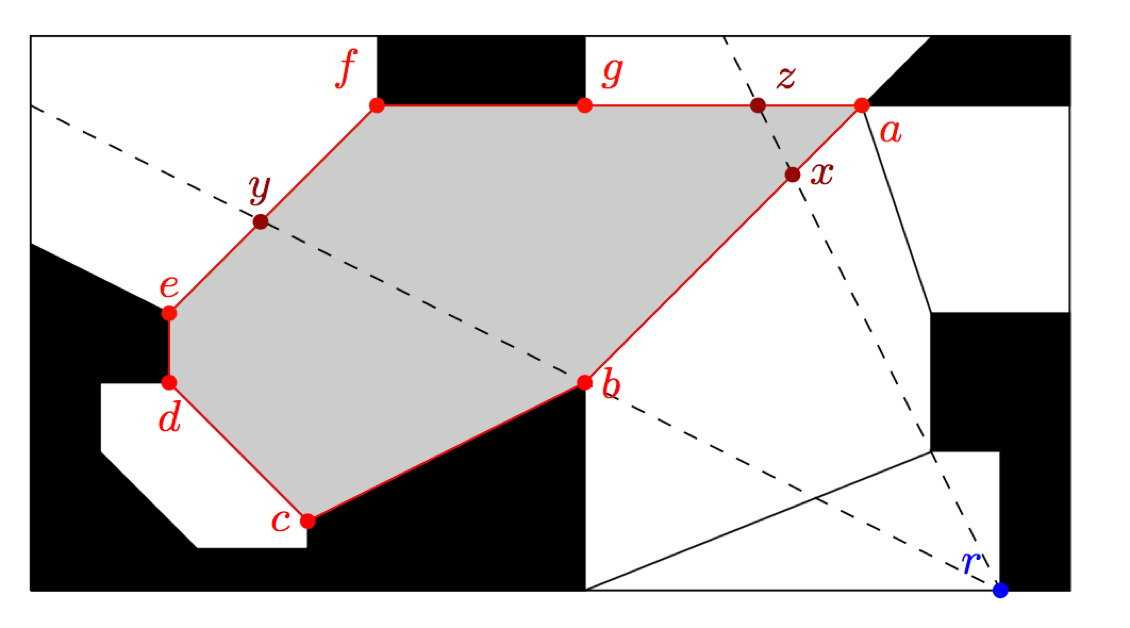
\includegraphics[width=.6\linewidth]{pic/suc.png}
    \caption{\small Example of successors from \cite{cuicompromise}.}
    \label{suc2}
\end{figure}

The version of \textit{Polyanya} we have just described is unlikely to be efficient. Without a
heuristic function for guidance, nodes can only be prioritized by the \textit{g-value} of their
root point, which is settled at the time of expansion. However, the \textit{g-value} does not
reflect the distance between the root and its corresponding interval. For example, in
Figure~\ref{suc2}, all observable successors would have the same expansion priority. Thus we
may expand many nodes, all equally priomising but having distant intervals, and all before
reaching a nearby target node with a slightly higher \textit{g-value}.

Another naive adaption is repeatedly calling an unmodified point-to-point \textit{Polyanya}
search, from the query point and to each target, let's call this \textbf{\textit{brute-force
Polyanya}}, see in algorithm~\ref{brute}. It is obvious that this solution is
inefficient when targets are many, however, in chapter\ref{empirical} we will see it
outperforms other proposed algorithms in certain contexts. 
\begin{algorithm}[!htp]
  \input{./code/brute_polyanya.pseudo}
  \caption{Brute-force Polyanya}
  \label{brute}
\end{algorithm}
To deal with this problem we develop two online heuristics which can be fruitfully applied to OkNN:
\begin{itemize}
  \item The Interval Heuristic, which prioritizes nodes using the closest point from its
    associated interval.
  \item The Target Heuristic, which relies on a Euclidean nearest neighbour estimator to
    provide a target dynamically at the time of expansion.
\end{itemize}
Each of these heuristic is applied in the usual way compute a final expansion priority: 
$f(n) = \textit{g-value}(n) + \textit{h-value}(n)$. In the remainder of this chapter we explore
these ideas in turn.

\section{Interval Heuristic}\label{intervalh}
In some OkNN settings targets are myriad and one simply requires a fast algorithm to explore
the local area. This approach is in contrast to more sophisticated methods which apply spatial
reasoning to prune the set of candidates. The idea we introduce for such settings is simple and
can be formalised as follows:

\begin{definition}
  Given search node $(I, r)$, the Interval Heuristic computes a value $h_i(I, r)$ which
  is the minimal Euclidean distance from the root $r$ to the segment $I$.
\end{definition}

Applying the Interval Heuristic $h_i$ requires solving a simple geometric problem: finding the
closest point on a line. The operation has low constant time complexity and we apply
standard techniques. Algorithm~\ref{intervalsrc} shows an example.

\begin{algorithm}[!htb]
  \input{./code/interval.pseudo}
  \caption{Polyanya OkNN with interval heuristic}
  \label{intervalsrc}
\end{algorithm}

\begin{theorem}{\textbf{(consistency)}:}\label{nodesc}
  The $\textit{f-value}$ of successor node is not less than the $\textit{f-value}$ of the parent
  search node.
\end{theorem}

\begin{proof}
  Using the interval heuristic, when the successor is a search node, its \textit{f-value}
  can be interpreted as a lower-bound of the length of path from
  $s$ to any point on the segment $I$ through root $r$, and since it is generated by pushing
  away from the parent search node, its \textit{f-value} is larger than \textit{f-value}
  of the parent search node. If successor is a target node, the \textit{f-value} is the the length
  of the corresponding path and not less than the parent search node (the two values are equal 
  when the target is on the segment $I$).%$\square$
\end{proof}

\begin{corollary}
  Expanding a target node corresponds to finding a shortest path.
\end{corollary}

\begin{proof}
  As per Theorem~\ref{nodesc}, when a final node is expanded there exists
  no remaining candidate on the open list which can reach the node with a smaller $f$-value.
\end{proof}

\section{Target Heuristic}\label{targeth}
In some OkNN settings the set of target are few (i.e. sparse), or there is a filter on the
query, for example, the query is like "the nearest storage location where capacity $>=100$". 
In these cases, without a reasonable heuristic guide, it is possible to perform many redundant
expansions in areas where no nearest neighbor can exist, Figure~\ref{hv} shows an example. 
\begin{figure}[htp]
  \centering
  \begin{tikzpicture}[scale=0.8]
    %\coordinate (a) at (2, 6); 
\coordinate (a) at (0, 7);
\coordinate (b) at (8, 7); 
\coordinate (c) at (6, 5); 
\coordinate (d) at (1, 3);
\coordinate (e) at (4, 3);
\coordinate (f) at (4, 2);
\coordinate (g) at (7, 4);
\coordinate (h) at (7, 2);
%\coordinate (i) at (9, 0);
\coordinate (i) at (10, 0);
\coordinate (j) at (5, 2);
\coordinate (k) at (0, 7);
\coordinate (l) at (0, 0);
\coordinate (m) at (10, 0);
\coordinate (n) at (10, 7);
\coordinate (q) at (3, 4);
\coordinate (Q) at (3, 4);
\coordinate (t) at (9, 3);
\coordinate (o) at (7.5, 5.5);

\newcommand{\nodelabel}[2] {
    \node[fill,circle,scale=0.25,label=#2:$#1$,color=red] at (#1) {$#1$};
}

\newcommand{\medge}[2]{
    \draw[gray,thick] (#1)--(#2);
}

\newcommand{\vgedge}[2]{
    \draw[black,thick] (#1)--(#2);
}

\newcommand{\drawVs}{
    %\nodelabel{a}{above}
    \nodelabel{b}{below}
    \nodelabel{c}{below}
    
    %\nodelabel{d}{left}
    \nodelabel{e}{right}
    \nodelabel{f}{below}
    
    \nodelabel{g}{above}
    \nodelabel{h}{below}
    %\nodelabel{i}{below}
}

\newcommand{\drawmeshs}{
    \medge{a}{k},\medge{a}{d},\medge{a}{b},\medge{a}{c}
    \medge{b}{c},
    \medge{c}{g}
    \medge{d}{f},\medge{d}{l},\medge{d}{e}
    \medge{l}{f}
    \medge{e}{c},\medge{e}{f}
    \medge{f}{h}
    \medge{g}{h},\medge{g}{b}
    \medge{h}{i}
}

\newcommand{\drawobstacles}{
    \fill[black] (a)--(b)--(c)--cycle;
    \fill[black] (g)--(h)--(i)--cycle;
    \fill[black] (d)--(e)--(f)--cycle;
}

\newcommand{\drawstart} {
    % \fill[blue] (q) circle[radius=.5ex];
    % \node[above] at (q) {$q$};
    \node[fill,circle,scale=0.25,label=above:$q$,color=blue] at (q) {$q$};

}

\newcommand{\drawend}{
    \fill[blue] (t) circle[radius=.5ex];
    \node[above] at (t) {$t$};
}

\newcommand{\drawboundary}{
    \draw[black, ultra thick] (k)--(n)--(m)--(l)--cycle;
}

\newcommand{\showvisible} {
    \fill[lightgray] (c)--(e)--(d)--(a);
    \nodelabel{e}{right}
    \nodelabel{c}{below}
    \drawstart;
}

\newcommand{\stepa} {
    \fill[lightgray] (c)--(e)--(d)--(a);
    \fill[lightgray] (c)--(g)--(h)--(f)--(e);
    \draw[black, thin] (q)--(g);
    \draw[green, very thick] (e)--(c);
    \drawstart
    \drawVs
}

\newcommand{\stepb} {
    \fill[lightgray] (c)--(e)--(d)--(a);
    \fill[lightgray] (c)--(g)--(h)--(f)--(e);
    \fill[lightgray] (c)--(g)--(b);
    \draw[black, thin] (q)--(g);
    \draw[green, very thick] (e)--(c);
    \draw[black, thin] (g)--(t);
    \draw[black, thin] (q)--(g);
    \draw[green, very thick] (g)--(c);
    \draw[green, very thick] (g)--(b);
    \drawstart
    \drawend
    \drawVs
}

\newcommand{\polyanyaexpand}{
    \draw[black,very thin, dashed] (q)--($(q)!5cm!(e)$);
    \draw[black,very thin, dashed] (q)--($(q)!5cm!(c)$);
    \draw[orange!50, line width=3pt] (j)--(h);
    \draw[orange!50, line width=3pt] (h)--(g);
    \draw[orange!50, line width=3pt] (g)--(c);
    \draw[cyan, line width=3pt] (e)--(f);
    \draw[cyan, line width=3pt] (f)--(j);
}

\newcommand{\drawVG}{
    \vgedge{a}{d},\vgedge{a}{e},\vgedge{a}{g},\vgedge{a}{h}
    \vgedge{b}{g},\vgedge{b}{m}
    \vgedge{c}{d},\vgedge{c}{e},\vgedge{c}{g},\vgedge{c}{f},\vgedge{c}{h}
    \vgedge{d}{l},\vgedge{d}{g}
    \vgedge{e}{h},\vgedge{e}{n}
    \vgedge{f}{l},\vgedge{f}{h},\vgedge{f}{m}
    \vgedge{g}{n}
}
\newcommand{\drawmap}{
    \drawboundary
    \drawobstacles
    \drawmeshs
    \drawVs
    \drawstart
    \drawend
}

\newcommand{\intervalexpansion}{
    \drawboundary
    \drawobstacles
    \drawmeshs
    {\draw[green!50, line width=3pt, dashed] (e)--(d);}
    {\draw[green!50, line width=3pt, dashed] (d)--(a);}
    {\draw[green!50, line width=3pt, dashed] (a)--(c);}
    {\draw[green!50, line width=3pt, dashed] (e)--(c);}
    {\draw[green!50, line width=3pt, dashed] (d)--(l);}
    {\draw[green!50, line width=3pt, dashed] (e)--(f);}
    {\draw[green!50, line width=3pt, dashed] (f)--(j);}
    {\draw[green!50, line width=3pt, dashed] (j)--(h);}
    {\draw[green!50, line width=3pt, dashed] (g)--(h);}
    {\draw[green!50, line width=3pt, dashed] (c)--(g);}
    {\draw[green!50, line width=3pt, dashed] (g)--(b);}
    {\draw[black, line width=3pt] (q)--(g);}
    {\draw[black, line width=3pt] (g)--(t);}
    \drawstart
    \drawend 
    \drawVs
}

    \intervalexpansion
  \end{tikzpicture}
  \caption{\small Search space of Interval Heuristic:$q$ is query point,
  $t$ is a target, green dashed segments are the interval of expanded search nodes.
  From the figure we can see that the algorithm does unnecessary expansions in the direction that no target.}
  \label{hv}
\end{figure}
\noindent
In such cases more sophisticated spatial reasoning can help to prune the set of nearest
neighbours and guide the search. The idea we introduce for such settings can be formalised as
follows:
\begin{definition}\label{close}
  The closest target $t$ of a search node $n$ is $t \in T$ where $h_p(n, t)$ is minimum.
\end{definition}
We implement this idea as follow: 
When the relative location between targets and $r$ are in case 3 of the $h_p$,
instead of flipping targets, we flip $r$, and thus formed six areas as shown in Figure~\ref{fa}.
For $t \in areaA$, the \textit{h-value} is $d_e(r, a) + d_e(a, t)$;
for $t \in areaA'$, the \textit{h-value} is $d_e(r',a) + d_e(a, t)$,
and because $d_e(r', a) = d_e(r, a)$, we can combine $areaA$ and $areaA'$,
so we need to find the nearest neighbor of $a$ for $t \in areaA \cup areaA'$;
by the same reason, we can combine $areaB, areaB'$, so finally we formed four areas.
Then following the example, we may reason as follows:
\begin{figure*}[!hbt]
  \centering
  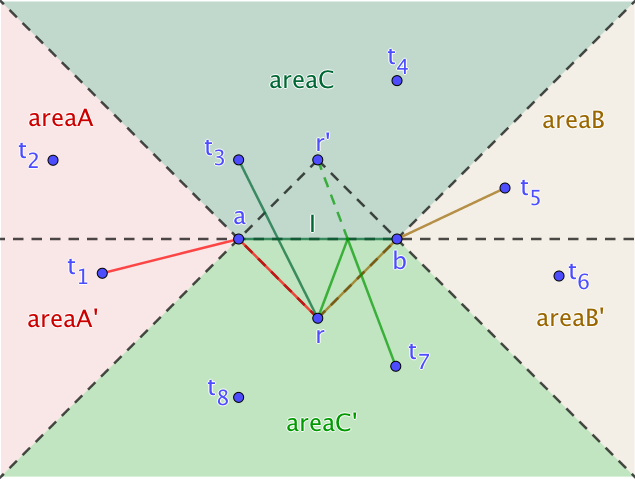
\includegraphics[width=.7\linewidth]{pic/heuristic.png}
  \caption{
    \small  
    \textbf{(i)} In $areaA \cup areaA'$, $t_1$ is the nearest to $a$;
    \textbf{(ii)} in $areaB \cup areaB'$, $t_5$ is the nearest to $b$;
    \textbf{(iii)} in $areaC$, $t_3$ is the nearest to $r$;
    \textbf{(iv)} in $areaC'$, $t_7$ is the nearest to $r'$; 
  }
  \label{fa}
\end{figure*}
\begin{itemize}
  \item Suppose the next nearest target $t$ is in $areaA \cup areaA'$ (equiv. $areaB \cup areaB'$).
    Then the optimal path must pass through the point $a$ (equiv. $b$) so the minimum $h$-value can be computed as:
    $\mathbf{min}\{d_e(r, a) + d_e(t, a)\}$ such that $t$ in $areaA \cup areaA'$
    (equiv. $areaB \cup areaB'$).
  \item Alternatively, suppose the next nearest target $t$ is instead in $areaC$.
    Then the optimal path must pass through a point $p$ in the open interval $(a, b)$.
    So the minimum $h$-value can be computed by minimising across all target points in $areaC$.
    A similar argument applies to a next nearest neighbour in $areaC'$ and we can apply a similar strategy,
    but only after mirroring the root point $r$ through the interval.
    This operation is in contrast to the admissible $f$-value estimate used by Polyanya in the point-to-point setting,
    which mirrors the target through the interval.
\end{itemize}
\noindent
Identifying the candidate target with minimum $h$-value in each of the four cases can be improved,
from a linear-time operation to NN query, by storing all of the
targets in a spatial data structure such as $R^*$-Tree~\cite{beckmann1990r}.
Thus we may compute a lower-bound estimate to the next nearest neighbour by minimising over
four candidates returned by the $R^*$-tree instead of evaluating all possible target points.

\subsection{Further Refinements}
We may notice that the Target Heuristic described thus far is potentially costly, requiring 
four NN query as compared to one constant time operation in the point-to-point case.
To mitigate this we could call the function less often. 
For example we can assign the nearest-neighbour candidate computed at the parent node to each successor.
We decide when to switch back to the Target heuristic using the point-to-point estimator:
if the value is different from parent to child we need to compute a new next nearest neighbour candidate.
We call this strategy \textit{lazy compute} and apply it throughout our experiments.
We find it reduces total running time by approximately 20\%.

\begin{lemma}\label{lazy-compute}
  Given search node $n=(I,r)$, its successor $n'=(I', r')$,
  and a target $t$ that minimises Euclidean distance to $n$ from among all possible candidates.
  Further suppose $h_e$(n, t) = $h_e$(n', t), where $h_e$ is the Polyanya point-to-point estimator.
  Then $t$ is also a target that minimises Euclidean distance to $n'$ among all possible candidates.
\end{lemma}

\begin{proof}
  If there is $t'$ closer to $n'$ than $t$, then $h_e(n', t') <
  h_e(n', t) = h_e(n, t)$, and because of Lemma~\ref{nodesc},
  $h_e(n, t') <= h_e(n', t')$, so,
  $t$ can't be the closest target of $n$, which is conflict with assumption. Thus, such $t'$
  doesn't exist.
  %$\square$
\end{proof}

Now, each search node has a target, and the search behavior should be broadly similar to 
the point-to-point setting.  But there is one significant difference:
when a nearest neighbor $t$ has been found, $t$ should no longer influence the search process.
Thus, we need to remove $t$ from search space and re-assign (i.e. update)
all search nodes in the queue which use $t$ as their closest target. 
To avoid exploring the entire queue we propose instead the following simple strategy: 
when such a node is dequeud from the open list, we apply $h_t$ to compute a new target
and we push the node back onto open all without generating any successors. 
We call this \textit{lazy reassign}.

\begin{lemma}\label{lazy-reassign}
  Let's call these search nodes who need reassignment \textbf{pseudo nodes}, and others
  \textbf{real nodes}. \textbf{Lazy reassign} never changes the relative order of real
  nodes in queue.
\end{lemma}

\begin{proof}
  Let $n_1, n_2$ be any pair of real nodes, and $s$ be any pseudo node.  After the reassignment,
  if $s$ become neither $n_1$ nor $n_2$, then inserting a third party search node has nothing to do with the relative order of $n_1$
  and $n_2$; otherwise, without the loss of generality, assume $s$ becomes $n_1$. If the relative
  order of them is $<n_2, s>$, then $f(n_2) <= f(s)$, and
  because of the definition~\ref{close}, we have $f(s) <= f(n_1)$, so
  relative order of $n_1, n_2$ doesn't change. Alternatively, if the relative order is $<s, n_2>$,
  then $n_1$  will be push to queue before $n_2$ pop out, so the relative order of $n_1, n_2$ doesn't
  change as well.%$\square$
\end{proof}

In Algorithm~\ref{hsearch}, we arrive at last at the final form of Polyanya OkNN. The algorithm
accepts either $h_v$ and $h_t$ as a heuristic function and has, in both cases, the same high level steps.

\begin{algorithm}[!ht]
  \input{./code/hsearch.pseudo}
  \caption{Polyanya OkNN}
  \label{hsearch}
\end{algorithm}

\section{Summary}
In this chapter, we start with two straightforward adaptions of point-to-point Polyany
and finally proposed two heuristics for the Polyanya OkNN algorithm.
For \textit{Interval Heuristic}, it supports multi-target by
removing $t$ from \textit{h-value}; for \textit{Target Heuristic}, it supports multi-target by
employing spatial index and computing closest target dynamically. Each heuristic has their
suitable scenario, in following chapters, we will evaluate their performance under different
scenarios (chapter~\ref{empirical})  and discuss some future improvements
(chapter~\ref{conclusionfuture}). 
